\chapter{Introduction and Theory}
%Give basic idea of the project and its content. Describe (and give references to) other relevant work in the literature.
%The goals of this project were to perform a Monte Carlo simulation of the Potts Model, to numerically generate the Density of States of a periodic and twisted lattice and investigate the behaviour of the interfaces that occur when a twist is introduced to the system, for a variety of Q states.
%These goals have been accomplished using a variety of techniques. 
%Including using both the Metropolis update algorithm and the Wang-Landau restricted sampling technique in a custom lattice solver written in C++.

This project studies the behaviour of interfaces that occur when a twist is added to a discrete state lattice.
The Potts Model as originally proposed was to reinterpret the Ising Model as a system of interacting spins.
Generalising such a system of interacting spins in 2 dimensions leads to a system of Q equally distributed angles.
\begin{equation}
\theta_n=\frac{2\pi n}{q}, n=1,2,...q
\end{equation}
Such as system has a Z(q) symmetry and the Hamiltonian can be written as.
\begin{equation}
\mathcal{H}=-\sum_{\left\langle ij \right\rangle} J(\theta_{ij})
\end{equation}
$J(\theta)$ is periodic in $2\pi$ and $\theta_{ij}$ is the difference in angles of the two neighbour states.
In this project we discard the planar Potts Model and focus on the standard Potts model that can be written in the form.
\begin{equation}
J(\theta_{ij})=J_c\delta_{Kr}(n_i,n_j)
\end{equation}
Where $n_i$ and $n_j$ are unit vectors for equal of the Q directions.
Taking the coupling constant $J_c$ to be equal to 1 we can write the Hamiltonian of the Potts Model used in this project as
\begin{equation}
\mathcal{H}=-\sum_{\left\langle ij \right\rangle} \delta_{Kr}(n_i,n_j)
\end{equation}

It is useful to look at the energy per unit volume.
The Minimum energy value per unit volume will be
\begin{equation}
E_{Min} = - \textrm{Number of Links per Lattice Site}
\end{equation}

You would expect the value for the Maximum energy per unit volume to be $0$ however this not quite the case due to the number of possible configurations that lead to the same system energy.
In other papers the issue of overlapping energy configurations is nullified by a scaling term. This leads to a slightly modified Hamiltonian.
\begin{equation}
\mathcal{H}=\sum_{\left\langle ij \right\rangle} \frac{1}{q} - \delta_{Kr}(n_i,n_j)
\end{equation}
However in this project the issue of incorrect scaling is dealt with by ignoring non-physical values so the Hamiltonian remains the same as before.

From the paper by F. Y. Wu the critical point on a square lattice in the anti-ferromagnetic case which the project focuses on can be written as \cite{RevModPhys.54.235}
\begin{equation}
\beta_c = \frac{1}{k_B T} = \ln\left(1+\sqrt{Q}\right)
\end{equation}

\section{Lattice}
It is impossible to perform computer simulations for infinite lattice sizes.
By using finite lattice sizes you introduce boundary effects that can, in particularly small lattices produce noise of significance.
For small lattices, it is often useful to introduce periodic boundary conditions so that this effect is diminished.
On a smaller lattice, there is a higher ratio of lattice sites close to the boundaries, this leads to a higher number of sites being affected by the non standard interactions that occur at these points.
In 2D the lattice is a regular euclidean grid where the sites in each direction are labelled between 0 and $L-1$.
In this project the following periodic boundary conditions are set on the lattice.
\begin{equation}
	\begin{split}
		s_{L,0} = s_{0,0}  \\
		s_{0,L} = s_{0,0}
	\end{split}
\end{equation}

In 3 dimensions by wrapping the boundaries of this 2 dimensional lattice you generate a torus. 

\begin{figure}[H]
	\centering
	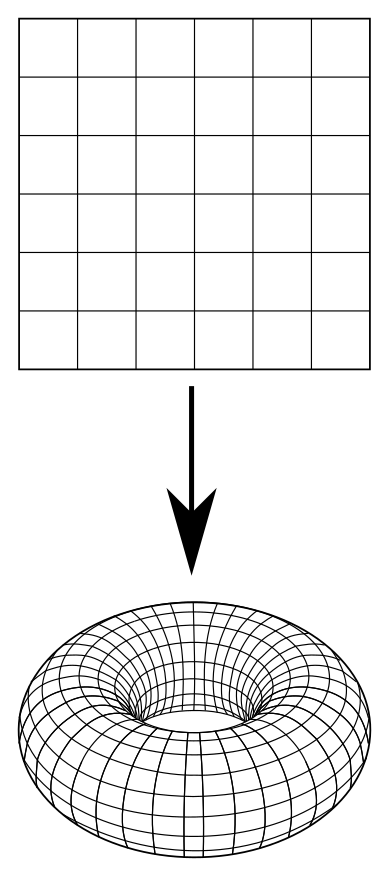
\includegraphics[width=0.25\textwidth]{2-Theory/latticetotorus.png}
	\caption{2 dimensional lattice transforming to torus in 3 dimensions under periodic boundary conditions}
\end{figure}

In this project I add a twist to the lattice in one axis then take separate measurements for this twisted lattice. To add a twist to the lattice in a single axis you need to relax the periodic condition in the axis of choice and define a boundary point. At this point every lattice site on the right has it's value set to be the lattice site on the left plus an arbitrary constant this new value is then put through the modulo operator to ensure that new Q states aren't generated during the process. The new state can be described as
\begin{equation}
s_{x,bp} = (s_{x,bp-1} + 1)\% Q
\end{equation}
Where x is any integer value between 0 and L-1, bp is the boundary point defined earlier.

\section{Observables}
	In this project, all of the results are given in terms of $\beta$ because it is the variable that is manipulated directly in the code.
	\begin{equation}
	\beta = \frac{1}{k_B T}
	\end{equation}		
	A simplification that can be made with ease involves setting the Boltzmann constant $k_B$ to be 1.
	
	\subsection{Magnetisation}
	Spontaneous Magnetisation is also known as the Magnetisation in the absence of an external Magnetic field. At high $\beta$, $\beta>\beta_{c}$, any of the lattice spin states can influence the states of its neighbours. In this lattice simulation the system has a net magnetisation even without a magnetic field. 
	At the critical point, $\beta_c$, the Magnetisation of the system can no longer remain zero.
	We can define the Magnetisation as the sum of each individual spin states.
	\begin{equation}
		M=\sum_{i}^{V}\sigma_{i}
	\end{equation}
	However when calculating the magnetisation from the $\theta_{i}$ form the Magnetisation becomes
	\begin{equation}
		M=\sum_{i}^{V} e^{i\theta_i}
	\end{equation}

	\subsection{Specific Heat}
	In a general case, the Specific Heat C can be defined as
	\begin{equation}
	C_V = \left\frac{\partial E}{\partial T}\right|_V
	\end{equation}
	It is a measurable physical quantity based upon the ratio between the heat added to an object and the relating temperature change.
	
	The form I use for the program 
	\begin{equation}
		C_V = \beta^2 \left[ \left\langle E^2 \right\rangle - \left\langle E \right\rangle ^2 \right]
	\end{equation}

	\subsection{Magnetic Susceptibility}
	The Magnetic Susceptibility is a dimensionless value that shows how much an extensive parameter changes when an intensive parameter increases.
	In this simulation the magnetic susceptibility tells us how much the magnetisation changes by increasing the temperature.
	In this project I take measurements using this form.
	\begin{equation}
		\chi = \beta \left[ \left\langle M^2 \right\rangle - \left\langle M \right\rangle ^2 \right]
	\end{equation}

\section{Partition Function}
	You can describe the Partition function as
	\begin{equation}
	Z = \sum_{\left\lbrace i \right\rbrace}} e^{-\beta E_i} \equiv \sum_{i} g(E_i) e^{-\beta E_i}
	\end{equation}
	Where $\left\lbrace i \right\rbrace$ is a generic configuration and $g(E_i)$ is the Density of States.
	Traditional approaches to calculate the Partition Functions through simulation have exponential fluctuations in volume, as such I used the algorithm proposed by F. Wang and D. P. Landau \cite{PhysRevLett.86.2050}.
	\begin{enumerate}
		\item Starting with any lattice configuration
		\item Choose a random site and change to a random value
		\item Accept the change with probability
		\begin{equation}
		P = min\left\lbrace \frac{g(E_{old})}{g(E_{new})},1 \right\rbrace
		\end{equation}
		If rejected revert the change.
		\item Update g(E_{new})
		\item Set $E_{old} =E_{new}$ and repeat from 2 until g(E) has converged.
	\end{enumerate}

	Performing this algorithm until the values converge allows for the reconstruction of the Density of States, which can then be used to calculate the Partition Function.
	In this project I calculate the Partition Function for both a regular Periodic Lattice and a Twisted Lattice for the various grid sizes chosen to study.

\section{Interfaces}
The Free Energy of a thermodynamic system is defined to be
\begin{equation}
F = -k_B T \ln{Z}
\end{equation}
To find the Free Energy of the Interface you need to take the logarithm of the ratio the partition functions calculated for the Periodic Lattice and the Twisted Lattice.
This leads to the equation for the Interface Free Energy
\begin{equation}
F_{s} = -\log{\frac{Z^*}{Z}}-\log{L}
\end{equation}
Z is the partition function of the periodic lattice, $Z^*$ is the partition function of the twisted lattice. Because the Interface can form at L points in the axis with the twist condition this needs to be subtracted to provide an accurate representation \cite{1111.4832}.
From the Interface Free Energy you can calculate the interface tension
\begin{equation}
\sigma = \lim_{L \to \infty} \frac{F_s}{V_{D-1}}
\end{equation}